%
% ---
% id : "electrotechnique_puissance_20260429_598"
% title : "Calculs moteur triphasé et pompe"
% domain : "Électrotechnique"
% subdomain : "Puissance"
% tags : ["moteur", "triphasé", "rendement", "facteur de puissance", "énergie", "puissance active", "puissance réactive", "ts"]
% difficulty : 2
% ---
\documentclass[a4paper,11pt,answers,addpoints]{exam}
% ---------------------------------------------------------
% LANGUE, ENCODAGE, FONTS
% ---------------------------------------------------------
\usepackage[utf8]{inputenc}

% ---------------------------------------------------------
% GÉOMÉTRIE ET MISE EN PAGE
% ---------------------------------------------------------
\usepackage[left=1.7cm,right=1.5cm,top=2cm,bottom=1cm]{geometry}
%\usepackage{a4wide}
\usepackage{microtype}      % Meilleure répartition du texte
\usepackage{float}          % Positionnement [H]
\usepackage{needspace}      % Saut conditionnel intelligent

% Éviter les veuves/orphelines (optionnel, à décommenter si besoin)
% \widowpenalty=10000
% \clubpenalty=10000

% Espacement vertical flexible
\raggedbottom
\setlength{\parskip}{0.5em plus 0.2em minus 0.1em}
\setlength{\parindent}{0pt}

% ---------------------------------------------------------
% MATHÉMATIQUES
% ---------------------------------------------------------
\usepackage{amsmath, amssymb, bm, esvect}

% Vecteurs
\newcommand{\V}{\overrightarrow}
\def\vect#1{\overrightarrow{\strut#1}}
\providecommand{\Degrees}[0]{\ensuremath{^\circ}}

% ---------------------------------------------------------
% UNITÉS ET GRANDEURS (SIunitx)
% ---------------------------------------------------------
\usepackage{siunitx}
\sisetup{output-decimal-marker={,}}
\DeclareSIUnit \var {var}
\DeclareSIUnit \VA {VA}
\DeclareSIUnit \kVA {kVA}
\DeclareSIUnit[quantity-product={}] \degree{\text{\textdegree}}

% ---------------------------------------------------------
% GRAPHIQUES : TikZ + CircuitikZ + PGFPlots
% ---------------------------------------------------------
\usepackage{tikz}
\usetikzlibrary{
	arrows.meta,
	intersections,
	decorations.pathreplacing,
	positioning
}

\usepackage[european,straightvoltages,EFvoltages]{circuitikz}

\usepackage{tkz-fct}
\usepackage{pgfplots}
\pgfplotsset{compat=1.12}

% Symbole étoile-triangle personnalisé
\newcommand{\wye}{%
	\mathbin{\tikz[x=1ex,y=1ex]{%
			\draw[line width=.1ex] (0,0)--(45:1)--++(-45:1) (45:1)--++(0,1);
	}}%
}


\usepackage{sankey}

\pgfdeclarelayer{background}
\pgfdeclarelayer{foreground}
\pgfdeclarelayer{sankeydebug}
\pgfsetlayers{background,main,foreground,sankeydebug}


% ---------------------------------------------------------
% TABLEAUX
% ---------------------------------------------------------
\usepackage{tabularx}
\usepackage{tabu}

% ---------------------------------------------------------
% HYPERLIENS
% ---------------------------------------------------------
\usepackage[colorlinks=true,
menucolor=red,
breaklinks=true,
urlcolor=blue,
linkcolor=blue]{hyperref}

% ---------------------------------------------------------
% COMMANDES PERSONNELLES
% ---------------------------------------------------------
\newcommand\nomauteur{bdminasmorgul@protonmail.com}
\newcommand\dateTe{29.04.2026}
\newcommand\brancheTe{TS}

% ---------------------------------------------------------
% STYLE DE L'EXERCICE
% ---------------------------------------------------------
\pagestyle{headandfoot}
\firstpageheadrule
\runningheadrule

\firstpageheader{\brancheTe\ (\nomauteur)}{Élève : }{(\dateTe) \thepage/\numpages}
\runningheader{\brancheTe\ (\nomauteur)}{Élève : }{(\dateTe) \thepage/\numpages}

% Compteur en bas de page
\newcommand{\totalpointtts}{%
	\begin{tikzpicture}[remember picture, overlay]
		\node[anchor=south west, inner sep=0pt, outer sep=0pt]
		at ([xshift=0.5cm,yshift=0.5cm]current page.south west)
		{\rotatebox{90}{Total des points : \numpoints}};
	\end{tikzpicture}
}

\firstpagefooter{\totalpointtts}{}{}
\runningfooter{\totalpointtts}{}{}

% Réglages exam
\printanswers
\addpoints
\pointsinmargin
\bracketedpoints

% ---------------------------------------------------------
% LISTINGS (code)
% ---------------------------------------------------------
\usepackage{xcolor}
\usepackage{listings}

\lstdefinestyle{octavestyle}{
	language=Matlab,
	basicstyle=\ttfamily\small,
	keywordstyle=\color{blue},
	commentstyle=\color{green!50!black},
	stringstyle=\color{red},
	stepnumber=1,
	frame=single,
	breaklines=true,
	breakatwhitespace=true,
	tabsize=4
}

% ---------------------------------------------------------
% DOCUMENT
% ---------------------------------------------------------
\begin{document}
\unframedsolutions
\pointsinmargin
\bracketedpoints
\section*{Préparation TS PQ CFC ELMO, IELE, PELE}

	
\noindent Avant de répondre aux différentes questions ci-dessous, observer  le diagramme de Sankey illustrant les flux énergétiques.


\begin{center}
	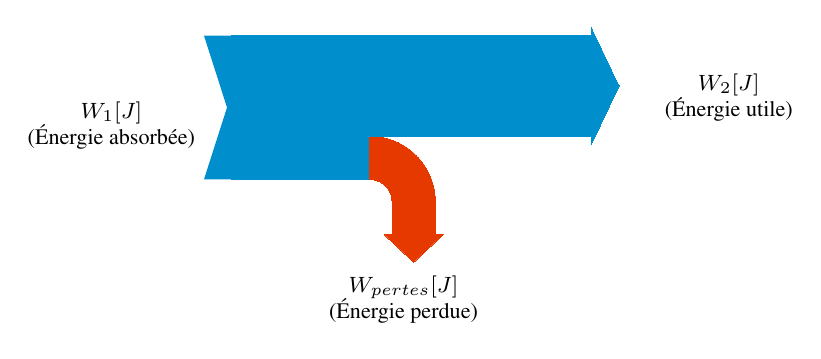
\begin{tikzpicture}
		% font choice
		\renewcommand\rmdefault{txr}\rmfamily\footnotesize
		\sisetup{
			round-mode=places,
			round-precision=1,
			add-decimal-zero,
		}
		
		\begin{sankeydiagram}
			\colorlet{energy}{blue!30!cyan!80!black}
			\colorlet{lost energy}{red!50!orange!90!black}
			\sankeyset{
				ratio=13em/100,
				minimum radius=1em,
				start style=arrow,end style=arrow,
				draw/.style={draw=none,line width=0},
				energy/.style={
					fill/.style={
						draw=energy,
						line width=0,
						fill=energy,
					}
				},
				lost energy/.style={
					fill/.style={
						draw=lost energy,
						line width=0,
						fill=lost energy,
					}
				}
			}
			\newcommand\abovelabel[2]{ % valname, label
				\node[xshift=-63pt,yshift=-44pt,anchor=south east,align=center,inner xsep=0] at (#1.left) {#2};
			}
			\newcommand\Punlabel[2]{ % valname, label
				\node[xshift=73pt,yshift=-34pt,anchor=south 		east,align=center,inner xsep=0] at (#1.left) {#2};
			}		
			\newcommand\belowlabel[2]{ % valname, label
				\node[anchor=south west,align=center,inner xsep=0, xshift=-23pt,yshift=-35pt] at 	(#1.south) {#2};
			}
			% Label de FIN (35) : inchangé
			\newcommand\energylabel[1]{ % valname
				\node[anchor=north east,text=energy,inner xsep=0] at (#1.right)
				{\num{\sankeygetnodeqty{#1}}};
			}
			
			% Label de DÉBUT (50) : corrigé avec overlay + ancre east
			\newcommand\energylabelstart[1]{ % valname
				\node[overlay, anchor=east, text=energy, inner xsep=0, yshift=-30pt, xshift=-61pt] at (#1.left)
				{\num{\sankeygetnodeqty{#1}}};
			}
			
			\newcommand\lostenergylabel[2]{ % valname, label
				\node[anchor=north,text=lost energy] at ([yshift=-3.5mm]#1.center)
				(value)
				{\num{\sankeygetnodeqty{#1}}};
				\node[anchor=north,inner sep=0,align=center] at (value.south) {#2};
			}
			\newcommand\lostenergylabelbottom[2]{ % valname, label
				\draw[draw=lost energy,dashed,thick]
				([yshift=-3mm]#1.center) coordinate (#1) -- ([yshift=-3mm]#1.center);
				\lostenergylabel{#1}{#2}
			}
			
			\newcommand\turnandstop[2]{ % valname, label
				\begingroup
				\sankeyset{lost energy}
				\sankeyturnright{#1}{90}
				\sankeynode{as=#1,name=#1-stop,at={#1 |- c}}
				\sankeyoutin{#1}{#1-stop}
				\sankeynode{as=#1-stop,name=#1}
				\sankeyend{#1}
				%			\lostenergylabel{#1}{#2}
				\endgroup
			}
			
			\sankeynode{name=Co,quantity=50.0}
			\path (Co.right) ++(40mm,-7mm) coordinate (c);
			
			\sankeyset{fill/.style={fill=energy}}
			\sankeynodestart{name=a,quantity=50}
			\def\hshift{6.25em}
			\sankeyadvance[energy]{Co}{1*\hshift}
			\abovelabel{Co}{\textbf{$W_1[J]$}\\(Énergie absorbée)}
			
			% Appel de la nouvelle commande pour le 50
			%		\energylabelstart{Co}
			
			\sankeyfork{Co}{35/P2,15/Pg}
			\turnandstop{Pg}{$W_{pertes}[J]$}
			
			\sankeyadvance[energy]{P2}{1.6*\hshift}
			\Punlabel{P2}{\textbf{$W_2[J]$}\\(Énergie utile)}
			
			% Commande d'origine pour le 35
			%		\energylabel{P2}
			
			\sankeyend[energy]{P2}
			
			\belowlabel{Pg}{\textbf{$W_{pertes}[J]$}\\(Énergie perdue)}
			
		\end{sankeydiagram}
		
	\end{tikzpicture}
\end{center}
\begin{questions}
\question Un moteur triphasé est utilisé pour entraîner une pompe industrielle. Les caractéristiques nominales indiquées sur sa plaque signalétique sont les suivantes : $P_2 = \qty{11}{[\kilo\watt]}$, $U = \qty{400}{[\volt]}$, $\cos \varphi = \qty{0,85}{}$ et un rendement $\eta = \qty{88}{[\%]}$. Le moteur fonctionne à pleine charge pendant une durée $t = \qty{8}{[\hour]}$.

\begin{parts}
	\part[3] Calculer la puissance active $P_1$ absorbée par le moteur sur le réseau~?
	\part[3] Déterminer l'intensité du courant de ligne $I$ consommé~?
	\part[3] Calculer la puissance réactive $Q$ fournie par le réseau~?
	\part[3] Quelle est l'énergie électrique $W$ consommée en kilowattheures durant cette période~?
	\part[3] Si le prix du kilowattheure est de \qty{0,25}{[CHF/\kilo\watt\hour]}, quel est le coût d'exploitation pour ces \qty{8}{[\hour]} de fonctionnement~?
\end{parts}
\vspace{0.5em}
\needspace{35\baselineskip}
\begin{solution}
	\begin{align*}
		\text{a) Calcul de la puissance absorbée } P_1 \text{ :} & \\[6pt]
		\eta &= \qty{88}{[\%]} = \qty{0,88}{} \\[6pt]
		P_1 &= \dfrac{P_2}{\eta} = \dfrac{\qty{11000}{[\watt]}}{\qty{0,88}{}} = \qty{12500}{[\watt]} = \qty{12,5}{[\kilo\watt]} \\[6pt]
		\text{b) Calcul de l'intensité du courant de ligne } I \text{ :} & \\[6pt]
		I &= \dfrac{P_1}{U \cdot \sqrt{3} \cdot \cos \varphi} = \dfrac{\qty{12500}{[\watt]}}{\qty{400}{[\volt]} \cdot \sqrt{3} \cdot \qty{0,85}{}} \\[6pt]
		I &= \qty{21,23}{[\ampere]} \\[6pt]
		\text{c) Calcul de la puissance réactive } Q \text{ :} & \\[6pt]
		S &= \dfrac{P_1}{\cos \phi} = \dfrac{\qty{12500}{[\watt]}}{\qty{0,85}{}} = \qty{14705,88}{[\volt\ampere]} \\[6pt]
		Q &= \sqrt{S^2 - P_1^2} = \sqrt{(\qty{14705,88}{})^2 - (\qty{12500}{})^2} = \qty{7746,95}{[\var]} \\[6pt]
		\text{d) Calcul de l'énergie consommée } W \text{ :} & \\[6pt]
		W &= P_1 \cdot t = \qty{12,5}{[\kilo\watt]} \cdot \qty{8}{[\hour]} = \qty{100}{[\kilo\watt\hour]} \\[6pt]
		\text{e) Calcul du coût d'exploitation :} & \\[6pt]
		\text{Coût} &= W \cdot \text{Prix} = \qty{100}{[\kilo\watt\hour]} \cdot \qty{0,25}{[CHF/\kilo\watt\hour]} = \qty{25}{[CHF]} \\[6pt]
	\end{align*}
	\vspace{0.5em}
	\needspace{35\baselineskip}
	\begin{verbatim}
		% Télécharger OCTAVE depuis https://wiki.octave.org/Using_Octave et l'installer
		% Puis copier-coller le code dans OCTAVE
		
		% Données de l'exercice (Inspiré par la source 2025_TS_PELE)
		P2 = 11000;         % Puissance utile [W]
		U = 400;            % Tension réseau [V]
		cosphi = 0.85;      % Facteur de puissance
		eta = 0.88;         % Rendement
		t = 8;              % Temps de fonctionnement [h]
		prix_kwh = 0.25;    % Prix de l'énergie [CHF/kWh]
		
		% a) Puissance absorbée P1
		P1 = P2 / eta;
		
		% b) Courant de ligne I
		I = P1 / (U * sqrt(3) * cosphi);
		
		% c) Puissance apparente S et réactive Q
		S = P1 / cosphi;
		Q = sqrt(S^2 - P1^2);
		
		% d) Énergie consommée W
		W_kwh = (P1 / 1000) * t;
		
		% e) Coût
		cout = W_kwh * prix_kwh;
		
		% Affichage des résultats
		printf("Puissance absorbée P1 : %.2f [W]\n", P1);
		printf("Intensité du courant I : %.2f [A]\n", I);
		printf("Puissance réactive Q : %.2f [var]\n", Q);
		printf("Énergie consommée W : %.2f [kWh]\n", W_kwh);
		printf("Coût d'exploitation : %.2f [CHF]\n", cout);
	\end{verbatim}
\end{solution}
\end{questions}
\end{document}